%%%%%%%%%%%%%%%%%%%%%%%%%%%%%%%%%%%%%%%%%%%%%%%%%%%%%%%%%%%%%%%%%%%%%%%%%%%%%%%
%%                                                           ENERGY CALIBRATION
%%%%%%%%%%%%%%%%%%%%%%%%%%%%%%%%%%%%%%%%%%%%%%%%%%%%%%%%%%%%%%%%%%%%%%%%%%%%%%%
%%                                          forward electron energy calibration 



%______________________________________________________________________________
%                                    Energiekalibration der Vorwärts-Elektronen
%
\chapter{Energiekalibration der Vorwärts-Elektronen}
\label{energy_calibration}

\begin{quote}
    Die Energiekalibration des elektromagnetischen Kalorimeters für Elektronen 
    ist von essentieller Bedeutung für Messung der Vorwärts-Rückwärts-
    Asymmetrie. Dieses Kapitel beschreibt die Kalibration für Elektronen mit
    hohen Pseudorapiditäten. Dabei wird zunächst auf \development 
\end{quote}



%______________________________________________________________________________
%                                                                    Grundlagen
%
\section{Grundlagen}
\label{energy_calibration:grundlagen}
\begin{itemize}
    \item Messung der Energie mit Kalorimeter (Verweis auf Detektor Kapitel)
    \item Notwendigkeit der Energiekalibration (Benötigte Präzision für 
        Vorwärts-Rückwärts-Asymmetrie)
    \item Vorangegangene Schritte ( Calibration-Hits, Test-Beam-Runs, 3-Stufen)
    \item Was im folgenden passiert (Vorwärts-Kalibration, in-situ
        kalibration, was ist noch zu kalibrieren)
    \item Zusätzliches Material
\end{itemize}



%______________________________________________________________________________
%                                                      Beschreibung der Methode 
%
\section{Beschreibung der Methode}
\label{energy_calibration:beschreibung_der_methode}

\begin{itemize}
    \item \sout{Betrachteter Prozess, CF-Ereignisse}
    \item \sout{Definition der Korrektur-Faktoren}
    \item \sout{Annahmen (perfekte zentral-Elektronen)}
    \item \sout{Vereinfachung der Formeln und Extraktion}
    \item 2-stufige Exktraktion
    \item Selektion und Samples
    \item Fit-Modelle, Effizienzkurve
\end{itemize}

Für die Kalibration der Vorwärts-Elektronen betrachtet man den elektroschwachen
Zerfalls-Prozess $Z/\gamma^* \rightarrow ee$ eines Z-Bosons in zwei
Elektronen\footnote{Die Bezeichnung \textit{Elektron} wird hier und im
Folgenden synonym für Elektronen und Positronen verwendet}. Dabei werden nur
Ereignisse selektiert, in denen eines der beiden Elektronen im Zentral-Bereich,
das andere im Vorwärts-Bereich detektiert wird. Diese Einbeziehung der Zentral-
Elektronen ist aus mehreren Gründen notwendig. Zum einen stehen entsprechende
Elektron-Trigger\footnote{siehe hierzu Kapitel
\ref{experimenteller_aufbau:atlas_detector:trigger-system}}
nur im Zentral-Bereich zur Verfügung. Zum anderen wäre die Selektion von
Ereignissen mit beiden Elektronen im Vorwärts-Bereich, in hohem Maße von
Untergrund-Prozessen dominiert, bei denen andere Objekte, überwiegend Jets,
fälschlicherweise als Elektronen rekonstruiert werden\footnote{vgl. Kapitel
\ref{experimenteller_aufbau:elektronen_in_atlas}}.
Allerdings stellt die Hinzunahme der Zentral-Elektronen die Kalibration der
Vorwärts-Elektronen ab initio in die Abhängigkeit einer vorangegangen 
Kalibration der Zentral-Elektronen.

Im folgenden Abschnitt werden zunächst einige grundlegende Annahmen eingeführt
und die Kalibration-Konstanten für Vorwärts-Elektronen definiert.



\subsection{Definitionen und Annahmen}
\label{energy_calibration:beschreibung_der_methode:definitionen_und_annahmen}

Die invariante Masse zweier relativistischer Teilchen, deren Ruhemassen
gegenüber ihren Energien vernachlässigt werden können, ergibt sich aus
\begin{equation}
    \label{invariant_mass:basic}
    m = \sqrt{ 2 \cdot E_1 E_2 (1-\cos\theta_{12}) }
\end{equation}
Dabei bezeichnet $E_{1/2}$ die Energie des Teilchens 1 bzw. 2 und $\theta_{12}$
den Öffnungswinkel zwischen beiden. Für die hier beschriebene Kalibration der
Vorwärts-Elektronen identifiziert man o.B.d.A. die Energie des Elektrons im
Zentral-Bereich mit $E_1$ und die Energie des Vorwärts-Elektrons mit $E_2$.

Man definiert nun den Kalibrations-Faktor $\alpha_i$, der die Abweichung zischen
wahrer und gemessener Energie korrigiert, wobei als beste Schätzung für die
\textit{wahre Energie} die \acs{MC}-Simulation des betrachteten Prozesses
herangezogen wird:
\begin{equation}
    \label{definition:energy_scale}
    E_\text{(data)} = E_\text{(MC)} (1+\alpha_i)
\end{equation}
Der Index $i$ weist darauf hin, dass für verschiedene Bereiche des
EM-Kalorimeters unterschiedliche Kalibrationskonstanten gelten. Man wählt eine
Unterteilung in der Pseudorapidität $\eta$, da mögliche Unterschiede vor allem
durch nicht-simuliertes passives Material, welches die Elektronen vor ihrem 
Eintritt in das Kalorimeter passieren, verursacht werden. Die grundsätzlich
inhomogene Verteilung von Materie vor dem Kalorimeter ist in Abbildung
\ref{fig:extra_material} dargestellt.
\begin{figure}
    \centering
    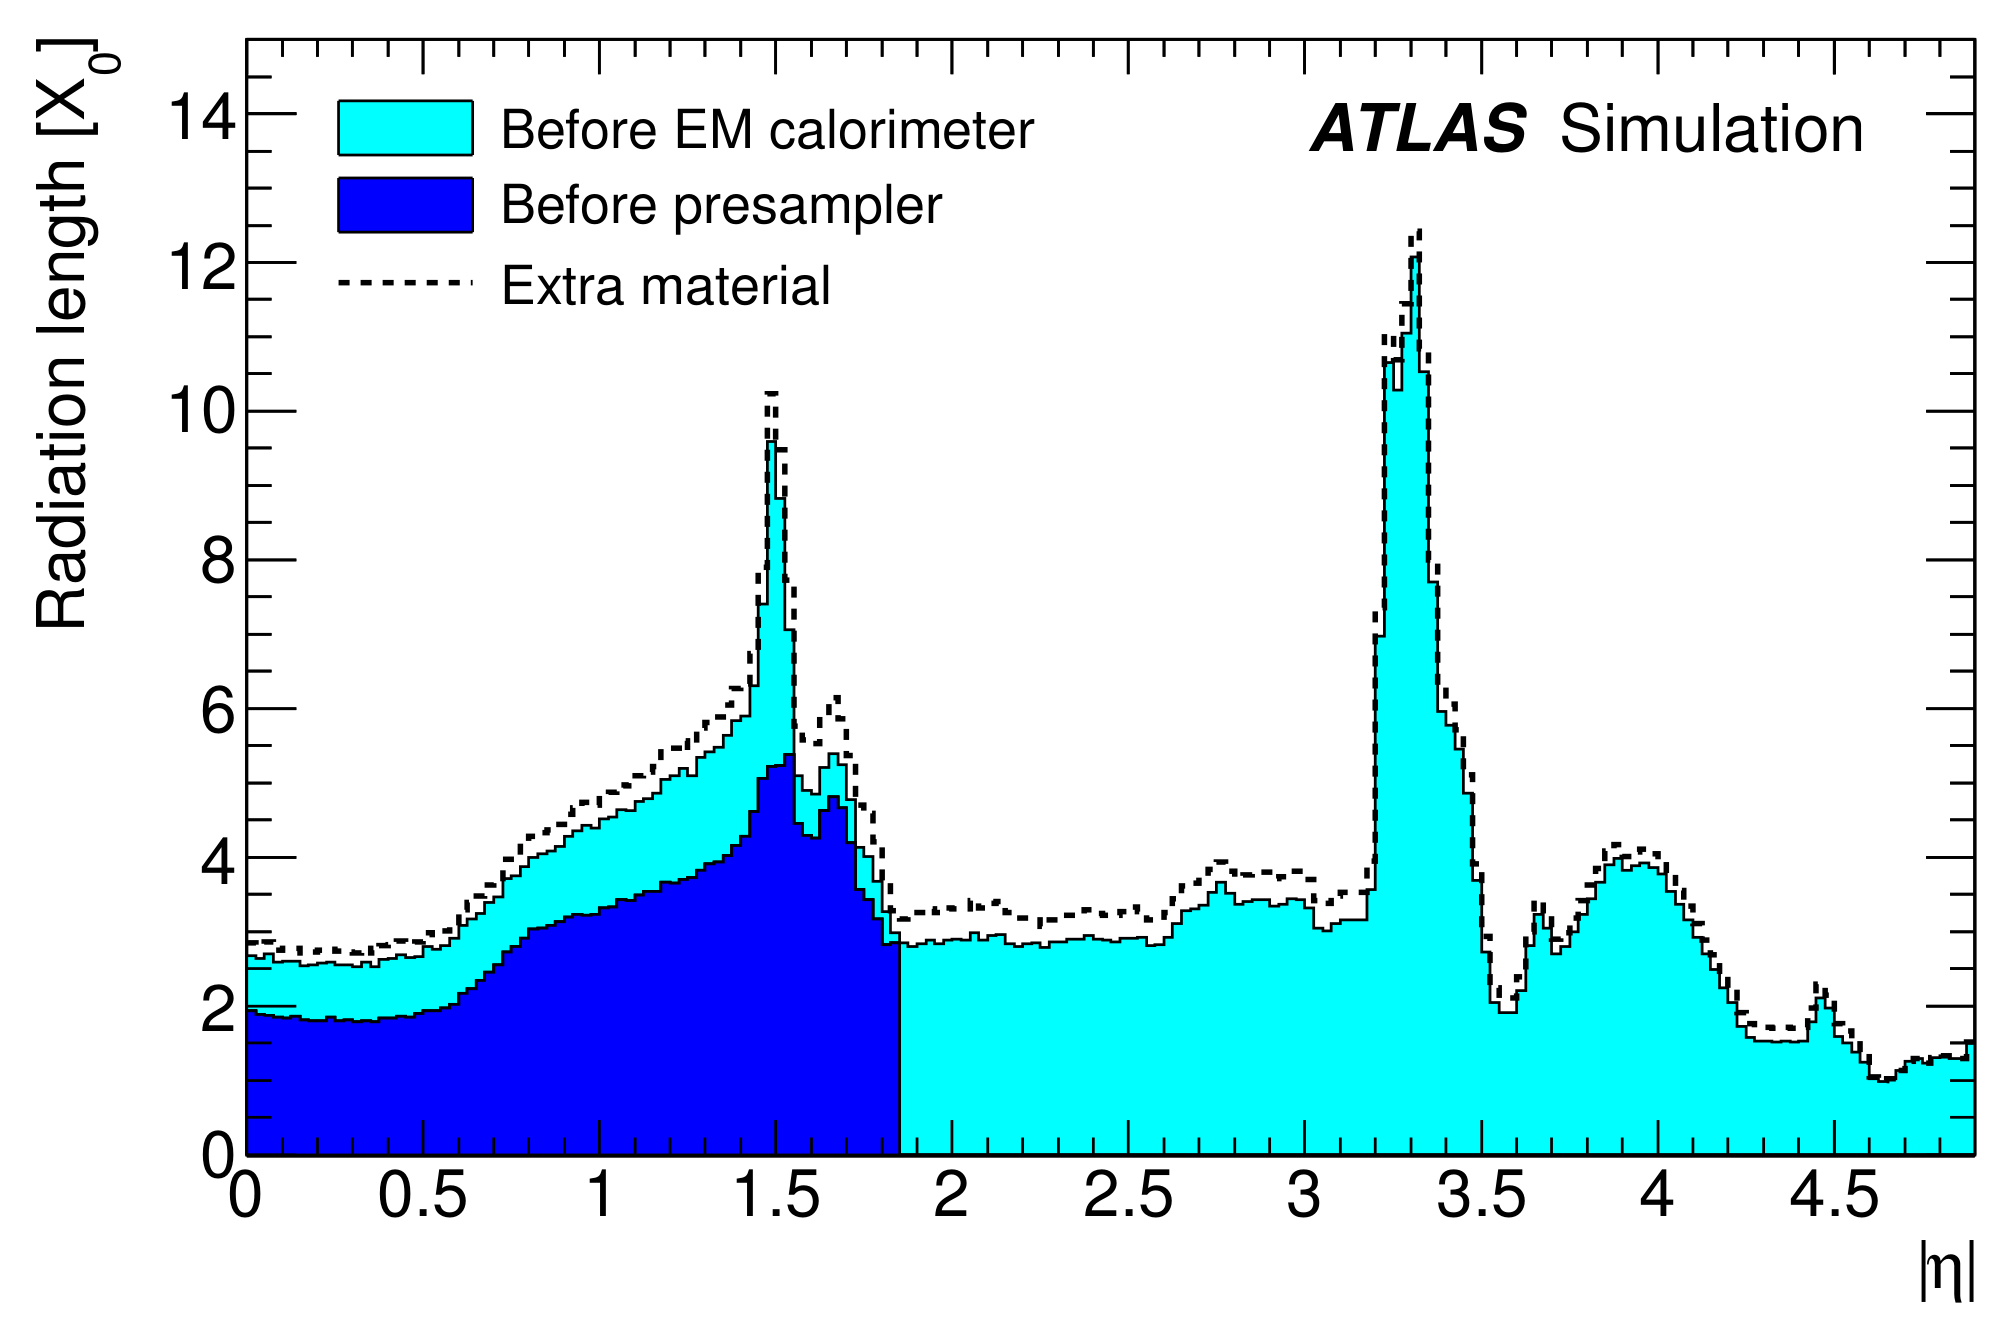
\includegraphics[width=0.7\textwidth]{img/extra_material}
    \caption[Material vor dem EM-Kalorimeter]
        {Die Menge an Material in Einheiten der Strahlungslänge $X_0$, die die
        Elektronen vor dem Kalorimeter durchfliegen, als Funktion der 
        Pseudorapidität $\eta$. Das zusätzliche Material wurde hier lediglich 
        zu systematischen Studien eingeführt und entspricht nicht der 
        tatsächlichen Verteilung. (Quelle: \cite{Aad:2011mk})}
    \label{fig:extra_material}
\end{figure}
Eine zusätzliche Unterteilung im Azimuthalwinkel $\phi$ wird nicht
vorgenommen, vielmehr geht man hier von einer isotropen Verteilung aus.

Wie bereits im einführenden Abschnitt \ref{energy_calibration:grundlagen}
erwähnt, werden die Elektronen im Zentral-Bereich als bereits perfekt
kalibriert angenommen, sodass gilt:
\begin{equation}
    \label{definition:perfect_central_electrons}
    E_\text{(data)}^\text{C} = E_\text{(MC)}^\text{C}
    \qquad \Longleftrightarrow \qquad
    \alpha_i^\text{C} = 0
    \qquad\qquad
    ^C : \text{zentral}
\end{equation}
Für die Messung der invarianten Masse (\ref{invariant_mass:basic}) des
\acs{CF}-Elektron-Paares folgt nun mit (\ref{definition:energy_scale}) und
(\ref{definition:perfect_central_electrons}):
\begin{align}
    m_\text{(data)}   &= \sqrt{ 2 \cdot E^C_\text{(data)} E^F_{\text{(data)}}
                         (1-\cos\theta)} 
                         \qquad ^C: \text{zentral}, \quad ^F: vorwärts
                         \nonumber \\[5pt]
                      &= \sqrt{ 2 \cdot E^C_\text{(MC)} E^F_{\text{(MC)}}
                         (1+\alpha^F_i)(1-\cos\theta)}
                         \nonumber \\[15pt]
    m^2_\text{(data)} &= 2 \cdot E^C_\text{(MC)} E^F_{\text{(MC)}}
                         (1+\alpha^F_i)(1-\cos\theta)
                         \nonumber \\[5pt]
                      &= m^2_\text{(MC)} (1+\alpha^F_i)
                         \label{eq:invariant_mass_sq}
\end{align}
Gleichung (\ref{eq:invariant_mass_sq}) liefert somit die Möglichkeit zur
Extraktion der Kalibrations-Faktoren
\begin{equation}
    \label{eq:extraction_alpha}
    \alpha_i^F = \frac{m^2_\text{(data)}}{m^2_\text{(MC)}} - 1
\end{equation}

Neben der der Korrektur der Energieskala in Daten, muss auf Seiten der
Simulation noch die Energieauflösung\footnote{siehe hierzu auch Kapitel
\ref{experimenteller_aufbau:atlas_detector:elektromagnetisches_kalorimeter}}
korrigiert werden. Wie eingangs bereits erwähnt ist die Auflösung des
Kalorimeters in der Simulation oftmals überschätzt, sodass eine zusätzliche
künstliche Verschmierung eingeführt wird um dies zu kompensieren.

Nach Gleichung (\ref{eq:calorimeter_resolution}) ist die Auflösung des
Kalorimeters gegeben durch 
\begin{equation}
    \left(\frac{\sigma_E}{E}\right)_\text{(MC)} =
        \frac{a}{\sqrt{E}} \oplus \frac{b}{E} \oplus c
\end{equation}
Der sognannte \textit{Sampling Term} $a$ wird dabei als von der Simulation
wohl modelliert angenommen, während der \textit{Rauschterm} $b$ aus Messungen
mit Test-Strahlen extrahiert wird (siehe \cite{1748-0221-5-11-P11006}). Jeder
zusätzliche Beitrag spiegelt sich im konstanten Term $c$ wieder. Dieser ist
nicht simulierbar und muss aus einem Vergleich mit der tatsächlichen Auflösung
in den Daten gewonnen werden. Dazu bildet man die partiellen Ableitungen von
Gleichung (\ref{invariant_mass:basic})
\begin{align}
    \frac{\del m}{\del E_i} \;&=\; \frac{1}{2m} \frac{m^2}{E_i}
        \;=\; \frac{m}{2 E_i} \qquad\quad i \in \{1,2\}
\end{align}
und bildet die Gaußsche Fehlerfortpflanzung für die Auflösung der invarianten
Masse:
\begin{align}
    \sigma_m^2 \;&=\; \left(\frac{\del m}{\del E_1}\sigma_{E_1}\right)^2 +
                      \left(\frac{\del m}{\del E_2}\sigma_{E_2}\right)^2
                \;=\; \frac{m^2}{4E_1^2}\sigma_{E_1}^2 +
                      \frac{m^2}{4E_2^2}\sigma_{E_2}^2
                      \nonumber \\[5pt]
    \Longleftrightarrow \quad
    \frac{4\sigma_m^2}{m^2} &= \frac{\sigma_{E_1}^2}{E_1^2} +
                               \frac{\sigma_{E_2}^2}{E_2^2}
\end{align}
Führt man nun für die Auflösung in der Simulation den konstanten Term $c$ ein
und vergleicht mit der Auflösung in den Daten so folgt:
\begin{align}
    &\sigma_{E_i}^2/E_i^2 \longrightarrow \sigma_{E_i}^2/E_i^2 + c_i^2
    \nonumber \\[10pt]
    &4\left(\frac{\sigma_m^2}{m^2}\right)_\text{(data)}
        = 4\left(\frac{\sigma_m^2}{m^2}\right)_\text{(MC)}
        + c_1^2 + c_2^2
\end{align}
Auch hier wird, wie schon bei der Energieskala, die Kalibration der
Zentral-Elektronen als perfekt angenommen, sodass $c_1 = 0$ gesetzt werden
kann. Desweiteren wird ebenfalls eine Unterteilung des Kalorimeters in der
Pseudorapidität $\eta$ vorgenommen\footnote{Es handelt sich um die selbe
Unterteilung, wie schon für die Kalibrations-Faktoren der Energieskala},
was durch den Index $i$ angezeigt wird.
\begin{align}
    \label{eq:extraction_constant_terms}
    4\left(\frac{\sigma_m^2}{m^2}\right)_\text{(data)}
        &= 4\left(\frac{\sigma_m^2}{m^2}\right)_\text{(MC)}
        + \left(c_i^F\right)^2
\end{align}
Gleichung (\ref{eq:extraction_constant_terms}) bietet somit die Möglichkeit zur
Extraktion der Verschmierungsterme
\begin{align}
    c_i^F &= \sqrt{ 4 \left[ \left(\frac{\sigma_m}{m}\right)^2_\text{(data)}
             - \left(\frac{\sigma_m}{m}\right)^2_\text{(MC)} \right] }
    \label{eq:constant_terms}
\end{align}



\subsection{Extraktionsmethode}
\label{energy_calibration:beschreibung_der_methode:extraktionsmethode}
Nachdem nun die notwendigen Definitionen und Annahmen zur Exktraktion der
Kali\-brations-Faktoren getroffen wurden, kann eine Prozedur zu deren
Bestimmung entwickelt werden.

Es müssen die Energieskalen\footnote{Der obere Index $F$ an den
Kalibrationsfaktoren wird im Folgenden der Einfachheit halber weggelassen}
$\alpha_i$ und die Verschmierungsterme $c_i$ für jeden Bereich in $\eta$ separat
gewonnen werden. Angepasst an die typischen Größen der Elektronschauer\footnote
{vlg hierzu auch Kapitel\ref{experimenteller_aufbau:elektronen_in_atlas}} im
Kalorimeter hat sich folgene Unterteilung als sinnvoll erwiesen:
\begin{table}[h]
    \centering
    \begin{tabular}{|c|c|c|c|c|c|}
        \multicolumn{6}{c}{\textbf{EMEC}} \\
        \hline
        2.5 - 2.6 & 2.6 - 2.7 & 2.7 - 2.8 & 2.8 - 2.9 & 2.9 - 3.0 & 3.0 - 3.16
        \\ \hline
    \end{tabular}
    \vspace{10pt}

    \begin{tabular}{|c|c|c|}
        \multicolumn{3}{c}{\textbf{FCal}} \\
        \hline
        3.35 - 3.6 & 3.6 - 4.0 & 4.0 - 4.9 \\
        \hline
    \end{tabular}
    \caption{Unterteilung der Vorwärts-Kalorimeter in der Pseudorapidität
             $|\eta|$ zur Extraktion der Kalibrations-Konstanten}
    \label{tab:calibration_binning}
\end{table}

Hierbei wurde der Bereich zwischen $3.16 < |\eta| < 3.35$ exkludiert, da sich
hier der Übergangsbereich zwischen \acs{EMEC} und \acs{FCal} befindet.

Das grundlegende Prinzip zur Extraktion der Kalibrations-Faktoren besteht nun
darin, für jede Unterteilung des Kalorimeters (Tabelle
\ref{tab:calibration_binning}) die invarianten Massenspektren in Daten und
Simulation zu erstellen und mittels einer Kurvenanpassung analytischer
Funktionen die Werte für Masse und Auflösung aus den Gleichungen
(\ref{eq:extraction_alpha}) und (\ref{eq:constant_terms}) zu bestimmen.

Zur Erstellung der invarianten Massenspektren werden Selektions-Schnitte
angewandt, die auf Seiten der Daten für eine Untergrund-Unterdrückung sorgen.
Tabelle \ref{tab:calibration_cuts} zeigt eine Übersicht über die Schnitte
auf Daten und Simulation.
\begin{savenotes}
\begin{table}[h]
    \centering
    \begin{tabular}{|c|c|}
        \hline
        \multicolumn{2}{|c|}{\textbf{Event basierte Schnitte}} \\
        \hline\hline
        \acs{GRL} (nur Daten) & (...)\_EgammaForward.xml\footnote{Verwendete \ac{GRL}:
            data12\_8TeV.periodAllYear\_DetStatus-v61-pro14-02
            \_DQDefects-00-01-00\_PHYS\_StandardGRL\_All\_Good
            \_EgammaForward.xml} \\
        \hline
        Trigger & e24vhi\_medium1 \textit{or} e60\_medium1 \\
        \hline
        primärer Vertex & $\geq 3$ \\
        \hline
    \end{tabular}
    \vspace{15pt}

    \begin{tabular}{|c|c|c|}
        \hline
        \multicolumn{3}{|c|}{\textbf{Elektron basierte Schnitte}} \\
        \textbf{Schnitt}&\textbf{Zentral-Elektron}&\textbf{Vorwärts-Elektron}\\
        \hline \hline
        Pseudorapidität & $|\eta| \leq 2.47$ & $2.5 \leq |\eta| \leq 4.9$ \\
        \hline
        Transversal-Impuls & $p_T > 25.0 \GeV$ & $p_T > 20.0 \GeV$ \\
        \hline
        Autor & 1 \textit{or} 3 & 8 \\
        \hline
        ID & \textit{tight++} & \textit{forward\_tight} \\
        \hline
        OQ & \multicolumn{2}{|c|}{- good object quality -} \\
        \hline
    \end{tabular}
    \caption[Übersicht über die bei der Energiekalibration verwendeten
        Selektion-Schnitte auf Daten und Simulation]
        {Übersicht über die bei der Energiekalibration verwendeten
        Selektions-Schnitte auf Daten (links) und Simulation (rechts)}
    \label{tab:calibration_cuts}
\end{table}
\end{savenotes}



%______________________________________________________________________________
%                                       Exktraktion der Kalibrations-Konstanten
%
\section{Extraktion der Kalibrations-Konstanten}
\label{energy_calibration:extraktion_der_kalibrations-konstanten}
\begin{itemize}
    \item Beispielhafte Fits
    \item Exktraktion der Energy-Scales
    \item Extraktion der Constant-Terms
    \item Systematiken
\end{itemize}



%______________________________________________________________________________
%                                                       Ergebnisse und Ausblick
%
\section{Ergebnisse und Ausblick}
\label{energy_calibration:ergebnisse_und_ausblick}
\begin{itemize}
    \item Zusammenfassung
    \item Diskussion ( Dominiert von Zentral-Skalen, Modell-Probleme )
    \item Verbesserungen ( Neue Zentral-Skalen, Template-Ansatz )
\end{itemize}


